\documentclass{acm_proc_article-sp}

\begin{document}

\title{A Comparative Study of the ESN and Elman Networks}

\numberofauthors{2}
\author{
\alignauthor
Rob Argue\\
       \affaddr{University of Maryland}\\
       \affaddr{Department of Computer Science}\\
       \email{rargue@cs.umd.edu}
% 2nd. author
\alignauthor
Joshua Bradley\\
       \affaddr{University of Maryland}\\
       \affaddr{Department of Computer Science}\\
       \email{jgbrad1@cs.umd.edu}
}
\maketitle

\section{Experiments}
In the analysis of our ESN three experiments were run. The initial experiment was parameter optimization of the ESN, and sought to explore the effects of network architecture and learning rule parameters on the performance of the model. Performance was measured as mean square error of ESN output and actual data for a test set of data which immediately suceeded the training data. Lastly a comparison of run time of the networks was conucted using the power consumption data set.

(CUT THIS OUT)
Three data sets were used for each of the experiments. The Mackey-Glass equation was used to generate the first set of data, which comprised a chaotic time series with no additional features. Stock market data [1] was used for a time series with several features. For the purpose of these experiments we took the finance sector portfolio to be the target data, and the other sectors to be features. A household power consumption data set [2] was used as an example of a time series with some missing data. All data was normalized to fall in the range $[-1,1]$. The expectation was that the ESN would perform best on the Mackey-Glass data and worst on the power consumption data.
(UP TO HERE)

Parameter optimizaation was run with the parameters $leakRate$, $reservoirSize$, $spectralRadius$, and $forgetSize$. For each data set each parameter was varied independantly of the others, and were held at default values of
$$leakRate = 0.5$$
$$reservoirSize = 100$$
$$spectralRadius = 0.5$$
$$forgetSize = 100$$

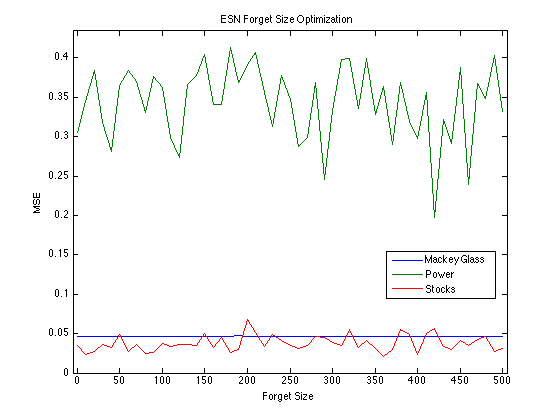
\includegraphics[scale=0.7]{ForgetSizeOptimization.png}
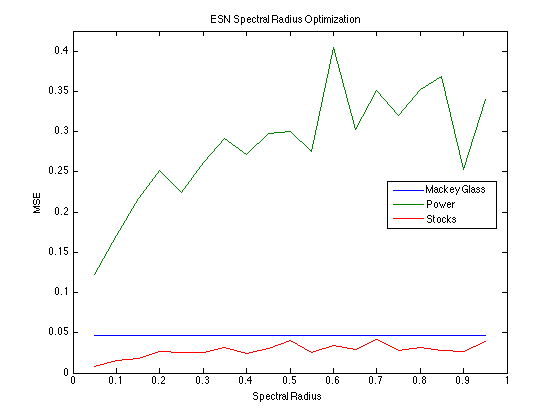
\includegraphics[scale=0.7]{SpectralRadiusOptimization.png}
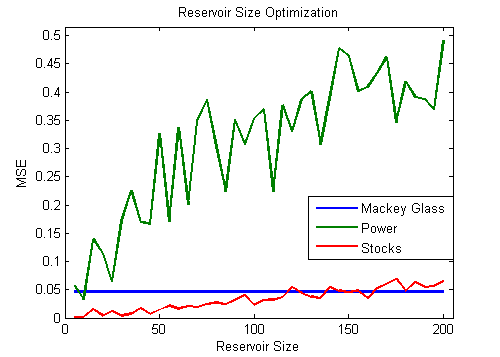
\includegraphics[scale=0.7]{ReservoirSizeOptimization.png}
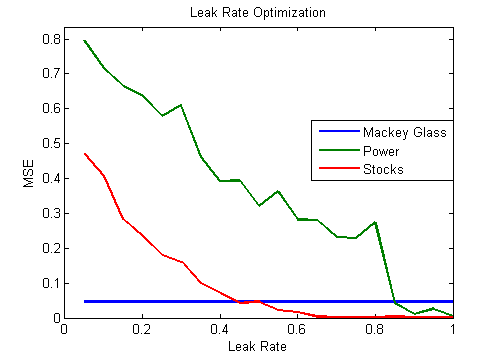
\includegraphics[scale=0.7]{LeakRateOptimization.png}

For all of the parameter, the Mackey-Glass performance stayed constant, which is consistant with what we saw for other networks. $forgetSize$ appearned to have little to no effect on the performance of the ESN, while the expectation was that there would be higher towards 0, which would quickly drop to a stable value. The ESN tended to perform better with smaller $spectralRadius$.  $reservoirSize$ similarly had a positive correlation with error, which is the opposite of expectation.  The decay of error with a higher $leakRate$ matched what we expected to happen.  Possible explanations for these results not matching our hypothesised results are (JOSH PUT SOMETHING HERE I DON'T KNOW).

In the second experiment we compared our ESN to other, commercially available neural networks. In particular we compared it to a feedforward network as a control, and to Elman and Jordan networks as examples of other recurrent nets. Matlab's Neural Network Toolbok was used for these networks. All three of the comparison networks were trained using RProp, and a best of three runs approach was taken in attempt to minimize the effect of outliers. We varied the size of the hidden layer (the reservoir in the case of our ESN) for some variety in architecture. The ESN used parameters optimized to each data set, while the other networks used default Matlab parameters in the interest of time.

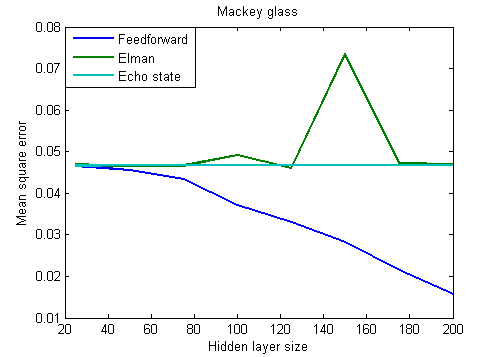
\includegraphics[scale=0.7]{mackey_plot.png}
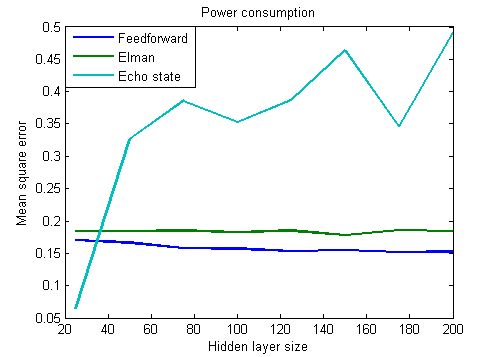
\includegraphics[scale=0.7]{power_plot.png}
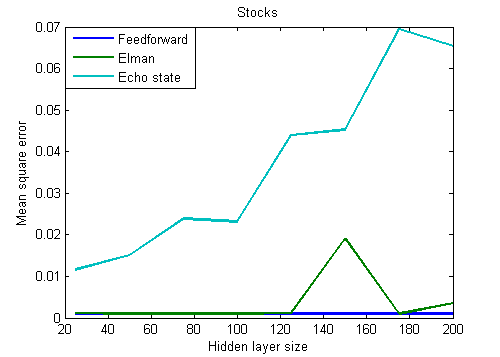
\includegraphics[scale=0.7]{stocks_plot.png}

The ESN performed best on the Mackey glass dataset, proving to be approximately equal to the Elman net, though with significantly higer consistancy, which matches with our expectations. For the power consumption dataset, the ESN performed somewhat poorer than the feedforward and Elman nets, with approximately double the error. On the stocks dataset the ESN performed significantly worse than the feedforward and Elman nets. This seems to indicate a general trend that the ESN performs more comparably on datasets which have fewer features, and instead tend to be more pure functions of time. Contrary to our initial hypothesis, did not seem to perform significantly worse compared to the other networks on the data set with missing data (the power consumption data set). 

The run time experiment was conducted under the same circumstances as the second experiment, however was only run on the power data set, and only one run was made for each data point.

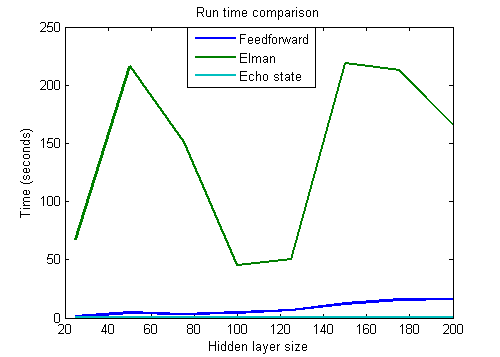
\includegraphics[scale=0.7]{time_plot.png}

The ESN took significantly less time to train, especially with a larger network size, running orders of magnitude faster than the Elman net, even at a small network size.

\section{Future Work}
Our ESN also has the ability to have output to reservoir connections, which we felt would be good to include for a comparison to Jordan nets. We were unable to finish debugging the Jordan nets in time to be able to conduct this comparison, so it is being left as future work. Additionally, parameter optimization for the Matlab nets should be performed, and other learning meathods for them would be interesting to investigate. Our ESN could also be adapted to work on multiple time series, and comparisons could be done with those.  

\section{Conclusions}
Our ESN performed reasonably well as compared to other simple recurrent nets. In general the ENS net tended to have somewhat worse performance, especially on featured data, but took a significantly shorter time to train, and was less prone to getting stuck in bad local minima, especially as compared to the Elman net. 
(WHAT ELSE DO YOU WANT TO SAY HERE?)

\end{document}